% Môn: Vật lý
% Lớp: 12
% Chương: Chương I. Vật lí nhiệt
% Bài: L12C1 Bài 6. Nhiệt hóa hơi riêng · Đọc và phân tích đồ thị quá trình chuyển thể
\dangbt{Đọc và phân tích đồ thị quá trình chuyển thể}
% ID: L12C1B1-TN-42
% Mức: NB
% ID: L12C1B1-91-TN


% ID: L12C1B1-TN-4
% Mức: NB
% ID: L12C1B1-97-TN
% ID: L12C1B1-97-TN
% Mức: NB
% ID: L12C1B1-97-TN
% Mức: NB
% ID: L12C1B1-97-TN


% ID: L12C1B1-TN-3
% Mức: NB
% ID: L12C1B1-100-TN
% ID: L12C1B1-100-TN
% Mức: NB
% ID: L12C1B1-100-TN
% Mức: NB
% ID: L12C1B1-100-TN
% ID: L12C1B1-100-TN
% Mức: NB
% ID: L12C1B1-100-TN
% Mức: NB
% ID: L12C1B1-100-TN


% ID: L12C1B1-TN-54
% Mức: TH
% ID: L12C1B1-131-TN
% ID: L12C1B1-131-TN
% Mức: TH
% ID: L12C1B1-131-TN
% Mức: TH
% ID: L12C1B1-131-TN
% ID: L12C1B1-131-TN
% Mức: TH
% ID: L12C1B1-131-TN
% Mức: TH
% ID: L12C1B1-131-TN
% ID: L12C1B1-131-TN
% Mức: TH
% ID: L12C1B6-124-TN
%=== Câu 44 ===%
\dangbt{Đọc và phân tích đồ thị quá trình chuyển thể}
\begin{ex}
% ID: L12C1B6-124-TN
% Mức: TH
	{\color{red}\footnotesize\ttfamily [L12C1B1-TN-54]}\par %HienID
	Bảng dưới đây ghi nhiệt độ của một chất theo thời gian khi được đun nóng liên tục:
	\begin{center}
		\begin{tabular}{|c|c|c|c|c|c|c|}
			\hline
			Thời gian (phút) & 0 & 2 & 4 & 6 & 8 & 10 \\
			\hline
			Nhiệt độ ($^\circ\mathrm{C}$) & 20 & 40 & 60 & 60 & 60 & 80 \\
			\hline
		\end{tabular}
	\end{center}
	Trong khoảng thời gian nào chất này đang nóng chảy?
	\choice
	{Từ phút thứ $0$ đến phút thứ $2$}
	{Từ phút thứ $2$ đến phút thứ $4$}
	{\True Từ phút thứ $4$ đến phút thứ $8$}
	{Từ phút thứ $8$ đến phút thứ $10$}
	\loigiai{
		Trong khoảng từ phút thứ $4$ đến phút thứ $8$, nhiệt độ của chất giữ nguyên ở $60^\circ\mathrm{C}$ dù vẫn được cung cấp nhiệt, đây chính là giai đoạn chất đang nóng chảy (nhiệt lượng dùng để phá vỡ liên kết mạng tinh thể chứ không làm tăng nhiệt độ).
		Kết luận: Chất đang nóng chảy trong khoảng từ phút thứ $4$ đến phút thứ $8$.
	}
\end{ex}

% ID: L12C1B1-TN-55
% Mức: NB
% ID: L12C1B1-132-TN
% ID: L12C1B1-132-TN
% Mức: NB
% ID: L12C1B1-132-TN
% Mức: NB
% ID: L12C1B1-132-TN
% ID: L12C1B1-132-TN
% Mức: NB
% ID: L12C1B1-132-TN
% Mức: NB
% ID: L12C1B1-132-TN
% ID: L12C1B1-132-TN
% Mức: NB
% ID: L12C1B6-125-TN
%=== Câu 45 ===%
\begin{ex}
% ID: L12C1B6-125-TN
% Mức: NB
	{\color{red}\footnotesize\ttfamily [L12C1B1-TN-55]}\par %HienID
	Dựa vào đồ thị nhiệt độ - thời gian của một chất rắn kết tinh khi nóng chảy, đoạn nằm ngang trên đồ thị cho biết điều gì?
	\choice
	{Nhiệt độ của chất đang tăng nhanh}
	{\True Chất đang nóng chảy, nhiệt độ không đổi dù vẫn nhận nhiệt}
	{Chất đã hoàn toàn chuyển sang thể lỏng và đang nguội đi}
	{Không có quá trình nào xảy ra}
	\loigiai{
		Đoạn nằm ngang trên đồ thị nhiệt độ - thời gian ứng với giai đoạn chất đang nóng chảy: nhiệt lượng cung cấp được dùng để phá vỡ cấu trúc mạng tinh thể (chuyển thể) chứ không làm tăng nhiệt độ, nên nhiệt độ giữ nguyên không đổi trong suốt giai đoạn này.
		Kết luận: Đoạn nằm ngang cho biết chất đang nóng chảy, nhiệt độ không đổi.
	}
\end{ex}

% ID: L12C1B1-TN-56
% Mức: TH
% ID: L12C1B1-133-TN
% ID: L12C1B1-133-TN
% Mức: TH
% ID: L12C1B1-133-TN
% Mức: TH
% ID: L12C1B1-133-TN
% ID: L12C1B1-133-TN
% Mức: TH
% ID: L12C1B1-133-TN
% Mức: TH
% ID: L12C1B1-133-TN
% ID: L12C1B1-133-TN
% Mức: TH
% ID: L12C1B6-126-TN
%=== Câu 46 ===%
\begin{ex}
% ID: L12C1B6-126-TN
% Mức: TH
	{\color{red}\footnotesize\ttfamily [L12C1B1-TN-56]}\par %HienID
	Một chất rắn kết tinh được đun nóng, đồ thị nhiệt độ - thời gian cho thấy: nhiệt độ tăng đều từ $20^\circ\mathrm{C}$ lên $60^\circ\mathrm{C}$ trong $4$ phút đầu, sau đó giữ nguyên ở $60^\circ\mathrm{C}$ trong $6$ phút tiếp theo (đang nóng chảy), rồi tiếp tục tăng. Nhiệt độ nóng chảy của chất này là bao nhiêu?
	\choice
	{$20^\circ\mathrm{C}$}
	{$40^\circ\mathrm{C}$}
	{\True $60^\circ\mathrm{C}$}
	{Không xác định được}
	\loigiai{
		Nhiệt độ nóng chảy của chất rắn kết tinh chính là giá trị nhiệt độ không đổi trong suốt đoạn nằm ngang của đồ thị, ở đây là $60^\circ\mathrm{C}$.
		Kết luận: Nhiệt độ nóng chảy của chất này là $60^\circ\mathrm{C}$.
	}
\end{ex}

% ID: L12C1B1-TN-57
% Mức: NB
% ID: L12C1B1-134-TN
% ID: L12C1B1-134-TN
% Mức: NB
% ID: L12C1B1-134-TN
% Mức: NB
% ID: L12C1B1-134-TN
% ID: L12C1B1-134-TN
% Mức: NB
% ID: L12C1B1-134-TN
% Mức: NB
% ID: L12C1B1-134-TN
% ID: L12C1B1-134-TN
% Mức: NB
% ID: L12C1B6-127-TN
%=== Câu 47 ===%
\begin{ex}
% ID: L12C1B6-127-TN
% Mức: NB
	{\color{red}\footnotesize\ttfamily [L12C1B1-TN-57]}\par %HienID
	Trên đồ thị nhiệt độ - thời gian của quá trình đun sôi một chất lỏng, đoạn đồ thị ứng với chất lỏng đang sôi có đặc điểm
	\choice
	{đường dốc lên, nhiệt độ tăng liên tục}
	{\True đường nằm ngang, nhiệt độ không đổi và bằng nhiệt độ sôi}
	{đường dốc xuống, nhiệt độ giảm dần}
	{đường gấp khúc bất kì, không tuân theo quy luật nào}
	\loigiai{
		Khi chất lỏng đang sôi, nhiệt độ của nó không đổi và giữ nguyên ở nhiệt độ sôi trong suốt quá trình, dù vẫn được cung cấp nhiệt (nhiệt lượng dùng để hóa hơi chất lỏng). Do đó đoạn đồ thị tương ứng là một đường nằm ngang.
		Kết luận: Đoạn ứng với chất lỏng đang sôi là đường nằm ngang tại nhiệt độ sôi.
	}
\end{ex}

% ID: L12C1B1-TN-22
% Mức: VD
% ID: L12C1B1-135-TN
% ID: L12C1B1-135-TN
% Mức: VD
% ID: L12C1B1-135-TN
% Mức: VD
% ID: L12C1B1-135-TN
% ID: L12C1B1-135-TN
% Mức: VD
% ID: L12C1B1-135-TN
% Mức: VD
% ID: L12C1B1-135-TN
% ID: L12C1B1-135-TN
% Mức: VD
% ID: L12C1B6-128-TN
%=== Câu 48 ===%
\begin{ex}
% ID: L12C1B6-128-TN
% Mức: VD
	{\color{red}\footnotesize\ttfamily [L12C1B1-TN-22]}\par %HienID
	Trộn $100\ \mathrm{g}$ nước đá ở $0^{\circ}\ \mathrm{C}$ với $100\ \mathrm{g}$ nước sôi ở $100^{\circ}\ \mathrm{C}$.  Hình nào sau đây mô tả quá trình thay đổi nhiệt độ theo thời gian của hệ trên?\\
	\begin{center}
		\resizebox{\textwidth}{!}{
			\begin{tabular}{cccc}
				\begin{tikzpicture}[very thick,>=stealth', scale=0.7,font=\footnotesize]
					\draw[->](0,0)--(3,0) node[below]{Thời gian};
					\draw[->](0,0)--(0,3) node[above]{Nhiệt độ ($^\circ \mathrm{C}$)};
					\filldraw (0,0) circle(1pt);
					\node[left] at (0,0) {$O$};
					\draw[red] (0,0)--(1,1);
					\draw[red] (0,2) node[left,black]{100} -- (1,1);
					\draw[red] (1,1)--(2,1);
					\node at (1.5,-1){Hình 1};
				\end{tikzpicture}
				&
				\begin{tikzpicture}[very thick,>=stealth', scale=0.7,font=\footnotesize]
					\draw[->](0,0)--(3,0) node[below]{Thời gian};
					\draw[->](0,0)--(0,3) node[above]{Nhiệt độ ($^\circ \mathrm{C}$)};
					\filldraw (0,0) circle(1pt);
					\node[left] at (0,0) {$O$};
					\draw[red] (1,0)--(1.5,0.5);
					\draw[red] (0,2) node[left,black]{100} -- (1.5,0.5);
					\draw[red] (1.5,0.5)--(2.3,0.5);
					\node at (1.5,-1){Hình 2};
				\end{tikzpicture}
				&
				\begin{tikzpicture}[very thick,>=stealth', scale=0.7,font=\footnotesize]
					\draw[->](0,0)--(3,0) node[below]{Thời gian};
					\draw[->](0,0)--(0,3) node[above]{Nhiệt độ ($^\circ \mathrm{C}$)};
					\filldraw (0,0) circle(1pt);
					\node[left] at (0,0) {$O$};
					\draw[red] (0,0)--(2.5,2);
					\draw[red] (0,2) node[left,black]{100} -- (2.5,0);
					\node at (1.5,-1){Hình 3};
				\end{tikzpicture}
				&
				\begin{tikzpicture}[very thick,>=stealth', scale=0.7,font=\footnotesize]
					\draw[->](0,0)--(3,0) node[below]{Thời gian};
					\draw[->](0,0)--(0,3) node[above]{Nhiệt độ ($^\circ \mathrm{C}$)};
					\filldraw (0,0) circle(1pt);
					\node[left] at (0,0) {$O$};
					\draw[red] (0,0)--(0.5,0.5);
					\draw[red] (0,2) node[left,black]{100} -- (1,2);
					\draw[red] (1,2)--(2,0.5);
					\draw[red] (0.5,0.5)--(2.5,0.5);
					\node at (1.5,-1){Hình 4};
				\end{tikzpicture}
			\end{tabular}
		}
	\end{center}
	\choice
	{Hình 1}
	{\True Hình 2}
	{Hình 3}
	{Hình 4}
	\loigiai{
		\begin{itemchoice}
			\item Hình 1 sai vì nhiệt độ của nước đá tăng ngay lập tức từ $0^{\circ}\ \mathrm{C}$. Trong thực tế, nước đá ở $0^{\circ}\ \mathrm{C}$ cần thu nhiệt để nóng chảy hoàn toàn trước khi nhiệt độ của nước sau khi tan có thể tăng lên.
			\item Hình 2 đúng vì:
			- Áp dụng đặc điểm của quá trình nóng chảy: Nước đá ở $0^{\circ}\ \mathrm{C}$ thu nhiệt để tan thành nước, trong suốt quá trình này nhiệt độ không thay đổi và duy trì ở $0^{\circ}\ \mathrm{C}$ (đoạn nằm ngang trên trục thời gian).
			- Áp dụng công thức tính nhiệt lượng tỏa ra: $Q_{\text{tỏa}} = m c \Delta t$, nước sôi ở $100^{\circ}\ \mathrm{C}$ tỏa nhiệt nên nhiệt độ giảm dần theo thời gian (đường đi xuống).
			- Sau khi đá tan hết, phần nước ở $0^{\circ}\ \mathrm{C}$ tiếp tục thu nhiệt để tăng nhiệt độ đến khi đạt trạng thái cân bằng nhiệt.
			\item Hình 3 sai vì đồ thị biểu diễn nhiệt độ của hai chất thay đổi tuyến tính mà không có giai đoạn chuyển thể (nóng chảy) của nước đá.
			\item Hình 4 sai vì diễn biến thay đổi nhiệt độ của các thành phần không đúng với quy luật truyền nhiệt trong hệ (nhiệt độ nước sôi không thể tăng thêm rồi mới giảm, và quá trình cân bằng không phù hợp).
		\end{itemchoice}
	}
\end{ex}

% ID: L12C1B1-DS-1
% Mức: VD
% ID: L12C1B1-140-DS
% ID: L12C1B1-140-DS
% Mức: VD
% ID: L12C1B1-140-DS
% Mức: VD
% ID: L12C1B1-140-DS
% ID: L12C1B1-140-DS
% Mức: VD
% ID: L12C1B1-140-DS
% Mức: VD
% ID: L12C1B1-140-DS
% ID: L12C1B1-140-DS
% Mức: VD
% ID: L12C1B6-129-DS
%=== Câu 53 ===%
\begin{ex}
% ID: L12C1B6-129-DS
% Mức: VD
	{\color{red}\footnotesize\ttfamily [L12C1B1-DS-1]}\par %HienID
	\immini{
		Hình bên là đồ thị biểu diễn sự thay đổi nhiệt độ theo thời gian trong quá trình chuyển từ thể rắn sang thể lỏng của chất rắn A và B.}
	{\begin{tikzpicture}[scale=0.8]
			\draw[->, thick] (0,0) -- (6.5,0) node[right] {Thời gian};
			\draw[->, thick] (0,0) -- (0,4) node[above] {Nhiệt độ};
			\node[below left] at (0,0) {0};
			
			% A: chất rắn vô định hình, nhiệt độ tăng liên tục
			\draw[blue, thick, smooth] plot coordinates {(0,1) (1,1.1) (2,3.1) (5,3.1) (6,3.1)};
			\node[blue, above] at (6,3.5) {A};
			
			% B: chất rắn kết tinh, có đoạn nằm ngang khi nóng chảy
			\draw[red, thick, smooth] plot coordinates {(0,1) (1,2.5) (4,2.5) (5,3.5)};
			\node[red, above] at (5,3.5) {B};
	\end{tikzpicture}}
	\choiceTF
	{\True Khi nung nóng liên tục, chất rắn A mềm đi và chuyển dần sang thể lỏng}
	{Chất rắn B không có cấu trúc tinh thể}
	{\True Chất rắn B có nhiệt độ nóng chảy xác định}
	{\True Chất rắn A là chất rắn vô định hình}
	\loigiai{\begin{itemchoice}
			\item  Vì A là chất rắn vô định hình.
			\item  Chất rắn B là chất rắn kết tinh nên có cấu trúc tinh thể.
			\item  Vì chất rắn B là chất rắn kết tinh.
			\item Chất rắn A là chất rắn vô định hình vì nhiệt độ tăng liên tục trong quá trình chuyển thể.
	\end{itemchoice}}
\end{ex}

% ID: L12C1B1-DS-2
% Mức: VD
% ID: L12C1B1-143-DS
% ID: L12C1B1-143-DS
% Mức: VD
% ID: L12C1B1-143-DS
% Mức: VD
% ID: L12C1B1-143-DS
% ID: L12C1B1-143-DS
% Mức: VD
% ID: L12C1B1-143-DS
% Mức: VD
% ID: L12C1B1-143-DS
% ID: L12C1B1-143-DS
% Mức: VD
% ID: L12C1B6-130-DS
%=== Câu 56 ===%
\begin{ex}
% ID: L12C1B6-130-DS
% Mức: VD
	{\color{red}\footnotesize\ttfamily [L12C1B1-DS-2]}\par %HienID
	Đồ thị biểu diễn sự thay đổi nhiệt độ của một lượng nước được đun sôi đến khi chuyển thể hoàn toàn thành hơi theo thời gian như hình vẽ.
	\begin{center}
		\resizebox{0.62\textwidth}{!}{
			\begin{tikzpicture}[
				line join=round,
				line cap=round,
				>=stealth,
				font=\footnotesize
				]
				
				% Khung nền
				\fill[gray!3, rounded corners=4pt] (-0.8,-0.8) rectangle (10.2,8.8);
				\draw[gray!60, rounded corners=4pt] (-0.8,-0.8) rectangle (10.2,8.8);
				
				% Lưới
				\draw[step=1, gray!25, very thin] (0,0) grid (9,8);
				
				% Trục tọa độ
				\draw[->, thick] (0,0)--(0,8.5) node[above left] {Nhiệt độ $\left(^{\circ}\mathrm{C}\right)$};
				\draw[->, thick] (0,0)--(9.8,0) node[below right] {Thời gian (phút)};
				
				% Gốc tọa độ
				\fill (0,0) circle (1.5pt);
				\node[below left] at (0,0) {$O$};
				
				% Nhãn trục Ox
				\foreach \x/\t in {0/0,1/2,2/4,3/6,4/8,5/10,6/12,7/14,8/16,9/18}
				{
					\node[below] at (\x,0) {\t};
				}
				
				% Nhãn trục Oy
				\foreach \y/\t in {1/20,2/40,3/60,4/80,5/100,6/120,7/140}
				{
					\node[left] at (0,\y) {\t};
				}
				
				% Các điểm
				\coordinate (A) at (0,1);
				\coordinate (B) at (2,5);
				\coordinate (C) at (7,5);
				\coordinate (D) at (8,7);
				
				% Đồ thị màu đỏ
				\draw[red!80!black, very thick] (A)--(B)--(C)--(D);
				
				% Đánh dấu điểm
				\fill[red!80!black] (A) circle (2pt);
				\fill[red!80!black] (B) circle (2pt);
				\fill[red!80!black] (C) circle (2pt);
				\fill[red!80!black] (D) circle (2pt);
				
				% Tên điểm
				\node[below right] at (A) {\large A};
				\node[above left] at (B) {\large B};
				\node[below] at (C) {\large C};
				\node[above right] at (D) {\large D};
				
				% Đường gạch phụ
				\draw[dashed, gray!70] (0,5)--(B);
				\draw[dashed, gray!70] (0,7)--(D);
				\draw[dashed, gray!70] (2,0)--(B);
				\draw[dashed, gray!70] (7,0)--(C);
				\draw[dashed, gray!70] (8,0)--(D);
				
			\end{tikzpicture}
		}
	\end{center}
	\choiceTF
	{\True Tại thời điểm ban đầu, nhiệt độ của nước là $20^{\circ}\ \mathrm{C}$}
	{Tốc độ chuyển động nhiệt của các phân tử nước sau $10\text{ phút}$ đun nước lớn hơn tốc độ chuyển động nhiệt của các phân tử nước sau $4\text{ phút}$ đun nước}
	{Sự sôi là sự hóa hơi xảy ra chỉ ở mặt thoáng của chất lỏng}
	{\True Đoạn $BC$ biểu diễn quá trình nước đang sôi. Trong giai đoạn này toàn bộ nhiệt lượng cung cấp cho nước dùng để hóa hơi nước}
	\loigiai{
		\begin{itemchoice}
			\item Dựa vào đồ thị, tại thời điểm bắt đầu khảo sát ($t = 0\text{ phút}$), đồ thị bắt đầu từ điểm $A$ có tung độ ứng với giá trị nhiệt độ là $20^{\circ}\ \mathrm{C}$.
			\item Tại thời điểm $4\text{ phút}$ và $10\text{ phút}$, nước đều ở trạng thái sôi với nhiệt độ không đổi là $100^{\circ}\ \mathrm{C}$. Vì tốc độ chuyển động nhiệt của các phân tử tỉ lệ thuận với nhiệt độ tuyệt đối của vật, nên tại hai thời điểm này tốc độ chuyển động nhiệt của các phân tử nước là như nhau.
			\item Theo đặc điểm của sự chuyển thể, sự sôi là quá trình hóa hơi diễn ra đồng thời ở mặt thoáng và cả trong lòng chất lỏng.
			\item Đoạn $BC$ trên đồ thị nằm ngang, tương ứng với nhiệt độ không đổi $100^{\circ}\ \mathrm{C}$, đây chính là quá trình sôi của nước. Trong suốt thời gian này, nhiệt lượng cung cấp cho nước không dùng để tăng nhiệt độ mà dùng để phá vỡ các liên kết giữa các phân tử nước nhằm thực hiện quá trình hóa hơi.
		\end{itemchoice}
	}
\end{ex}

% ID: L12C1B1-DS-7
% Mức: VD
% ID: L12C1B1-145-DS
% ID: L12C1B1-145-DS
% Mức: VD
% ID: L12C1B1-145-DS
% Mức: VD
% ID: L12C1B1-145-DS
% ID: L12C1B1-145-DS
% Mức: VD
% ID: L12C1B1-145-DS
% Mức: VD
% ID: L12C1B1-145-DS
% ID: L12C1B1-145-DS
% Mức: VD
% ID: L12C1B6-131-DS
%=== Câu 58 ===%
\begin{ex}
% ID: L12C1B6-131-DS
% Mức: VD
	{\color{red}\footnotesize\ttfamily [L12C1B1-DS-7]}\par %HienID
	
	\begin{wrapfigure}{r}{4cm}
		\vspace{-10pt}
		\centering
		\resizebox{0.7\linewidth}{!}{%
			\begin{tikzpicture}[>=stealth, thick]
				\draw [->] (0,0) -- (6.5,0);
				\draw [->] (0,0) -- (0,4.5);
				\draw[red] (0,0) [out = 80, in = -150] to (1,2) -- (3,2) [out = 10, in = -170] to (4.5,4) -- (6,4)
				node [left] at (0,2) {$17$}
				node [left] at (0,4) {$117$}
				node [left] at (0,0) {$O$}
				node [below] at (0.45,0) {$t_1$}
				node [below] at (2,0) {$t_2$}
				node [below] at (3.75,0) {$t_3$}
				node [below] at (5,0) {$t_4$}
				node [right] at (0,4.5) {Nhiệt độ $\left(^\circ \mathrm{C} \right) $}
				node [above] at (6,0) {Thời gian};
				\draw [dashed]
				(0,1.5) -- (0.45,1.5) -- (0.45,0)
				(0,2) -- (2,2) -- (2,0)
				(0,3) -- (3.75,3) -- (3.75,0)
				(0,4) -- (5,4) -- (5,0);
			\end{tikzpicture}
			
		}
		\vspace{-10pt}
	\end{wrapfigure}
	Khi làm thí nghiệm đun nóng một chất. Kết quả thí
	nghiệm, một học sinh vẽ được biểu diễn sự thay đổi
	nhiệt độ của chất đó theo thời gian như hình bên.
	\choiceTF
	{Tại thời điểm $t_2$, chất đang ở thể lỏng}
	{\True Nhiệt độ nóng chảy của chất là $17^\circ \mathrm{C}$}
	{Tại thời điểm $t_3$, chất đang ở cả thể rắn và thể lỏng}
	{Nhiệt độ sôi của chất này là $115^\circ \mathrm{C}$}
	
	\loigiai{\begin{itemchoice}
			\item Tại thời điểm $t_2$ chất đang ở cả thể rắn và thể lỏng.
			\item Trong quá trình chuyển thể, {\color{blue} nhiệt độ của cục nước đá tăng là sai vì  nhiệt độ của chất rắn không tăng lên mà thay vào đó, năng lượng được sử dụng để phá vỡ cấu trúc tinh thể và cung cấp động năng cho các phân tử}
			\item Tại thời điểm $t_3$ chất đang ở thể lỏng.
			\item Nhiệt độ sôi của chất này là $117^\circ \mathrm{C}$
	\end{itemchoice}}
\end{ex}

% ID: L12C1B1-DS-10
% Mức: VD
% ID: L12C1B1-146-DS
% ID: L12C1B1-146-DS
% Mức: VD
% ID: L12C1B1-146-DS
% Mức: VD
% ID: L12C1B1-146-DS
% ID: L12C1B1-146-DS
% Mức: VD
% ID: L12C1B1-146-DS
% Mức: VD
% ID: L12C1B1-146-DS
% ID: L12C1B1-146-DS
% Mức: VD
% ID: L12C1B6-132-DS
%=== Câu 59 ===%
\begin{ex}
% ID: L12C1B6-132-DS
% Mức: VD
	{\color{red}\footnotesize\ttfamily [L12C1B1-DS-10]}\par %HienID
	\immini[thm]
	{
		Đồ thị ở hình bên cho biết sự thay đổi nhiệt độ của một chất lỏng khi bị đun nóng cho đến khi sôi.
		\choiceTF
		{ \True Nhiệt độ sôi của chất lỏng là $\rm 80^\circ \mathrm{C}$}
		{ \True Trong quá trình sôi, nhiệt độ của chất lỏng không tăng}
		{ \True Nếu chất lỏng được đun nóng mạnh hơn (bởi nguồn nhiệt có công suất cấp nhiệt lớn hơn) thì đồ thị nhiệt độ của chất lỏng đó theo thời gian có độ dốc ban đầu tăng lên (nghĩa là chất lỏng sôi nhanh hơn)}
		{ Nếu chất lỏng được đun nóng mạnh hơn (bởi nguồn nhiệt có công suất cấp nhiệt lớn hơn) thì nhiệt độ sôi của chất lỏng có thể lớn hơn  $\rm 80^\circ \mathrm{C}$}}
	{
		\begin{tikzpicture}[>=stealth,scale=0.75,font={\footnotesize }]
			\draw[->,thick] (0,0)--(8,0) node [below] {Thời gian};
			\draw[->,thick] (0,0)--(0,5.5) node [right] {Nhiệt độ};
			\foreach \x/\xtext in {0/O,1/1,2/2,3/3,4/4,5/5,6/6}
			\draw[shift={(\x,0)}] (0pt,2pt) -- (0pt,-2pt) node[below] {$\rm \xtext$};
			\foreach \y/\ytext in {1/20,2/40,3/60,4/80}
			\draw[shift={(0,\y)}] (2pt,0pt) -- (-2pt,0pt) node[left] {$\rm \ytext$}; % đơn vị trục
			\draw[xstep=1, ystep=0.5, densely dashed,thin] (0,0) grid (7,4.5);
			\draw [domain=0:4, thick, smooth] plot (\x, -0.125*\x^2+1.125*\x+1.5);
			\draw [thick] (4,4)--(7,4);
			\draw (8,-1) node {$\left(\text{phút} \right) $};
			\draw (0.3,5) node [right] {$\left( \rm ^\circ \mathrm{C} \right) $};
	\end{tikzpicture}}
	\loigiai{\begin{itemchoice}
			\item Nhiệt độ sôi của chất lỏng là $\rm 80^\circ \mathrm{C}$ . Lúc sôi nhiệt độ của vật không tăng nữa.
			\item Trong quá trình sôi, nhiệt độ của chất lỏng không tăng.
			\item Nếu chất lỏng được đun nóng mạnh hơn (bởi nguồn nhiệt có công suất cấp nhiệt lớn hơn) thì đồ thị nhiệt độ của chất lỏng đó theo thời gian có độ dốc ban đầu tăng lên (nghĩa là chất lỏng sôi nhanh hơn).
			\item Nếu chất lỏng được đun nóng mạnh hơn (bởi nguồn nhiệt có công suất cấp nhiệt lớn hơn) thì nhiệt độ sôi của chất lỏng có thể lớn hơn $\rm 80^\circ \mathrm{C}$. Ở áp suất nhất định nhiệt độ sôi của vật là xác định.
	\end{itemchoice}}
\end{ex}

% ID: L12C1B1-DS-11
% Mức: VD
% ID: L12C1B1-147-DS
% ID: L12C1B1-147-DS
% Mức: VD
% ID: L12C1B1-147-DS
% Mức: VD
% ID: L12C1B1-147-DS
% ID: L12C1B1-147-DS
% Mức: VD
% ID: L12C1B1-147-DS
% Mức: VD
% ID: L12C1B1-147-DS
% ID: L12C1B1-147-DS
% Mức: VD
% ID: L12C1B6-133-DS
%=== Câu 60 ===%
\begin{ex}
% ID: L12C1B6-133-DS
% Mức: VD
	{\color{red}\footnotesize\ttfamily [L12C1B1-DS-11]}\par %HienID
	Một tinh thể bị nấu chảy thành chất lỏng nóng và sau đó nguội đi. Bảng bên dưới ghi lại nhiệt độ của mẫu chất lỏng nóng theo thời gian.
	
	\begin{center}
		\begin{tabular}{|>{\centering\arraybackslash}m{3cm}|
				>{\centering\arraybackslash}m{1.5cm}|
				>{\centering\arraybackslash}m{1.5cm}|
				>{\centering\arraybackslash}m{1.5cm}|
				>{\centering\arraybackslash}m{1.5cm}|
				>{\centering\arraybackslash}m{1.5cm}|
				>{\centering\arraybackslash}m{1.5cm}|
				>{\centering\arraybackslash}m{1.5cm}|}
			\hline
			Thời gian (phút) & 0 & 5 & 10 & 15 & 20 & 25 & 30 \\ \hline
			Nhiệt độ ($\rm ^\circ \mathrm{C}$) & 90 & 75 & 68 & 68 & 68 & 62 & 58 \\ \hline
		\end{tabular}
	\end{center}
	
	\choiceTF
	{ \True Tại phút thứ $5$, mẫu chất tồn tại ở thể lỏng}
	{ Trong khoảng thời gian từ phút thứ $10$ đến phút thứ $20$, mẫu chất lỏng đang nóng chảy}
	{ \True Nhiệt độ nóng chảy của tinh thể là $\rm 68^\circ \mathrm{C}$}
	{ Tại thời điểm phút thứ $15$, mẫu chất tồn tại ở thể rắn}
	\loigiai{
		\begin{itemchoice}
			\item Tại phút thứ $5$, mẫu chất tồn tại ở thể lỏng vì nhiệt độ còn lớn hơn $68^\circ \mathrm{C}$.
			\item Trong khoảng thời gian từ phút thứ $10$ đến phút thứ $20$, mẫu chất đang đông đặc, không phải nóng chảy.
			\item Nhiệt độ nóng chảy của tinh thể là $\rm 68^\circ \mathrm{C}$.
			\item Tại phút thứ $15$, mẫu chất đang tồn tại đồng thời ở thể rắn và thể lỏng.
		\end{itemchoice}
	}
\end{ex}

% ID: L12C1B1-DS-12
% Mức: VDC
% ID: L12C1B1-148-DS
% ID: L12C1B1-148-DS
% Mức: VDC
% ID: L12C1B1-148-DS
% Mức: VDC
% ID: L12C1B1-148-DS
% ID: L12C1B1-148-DS
% Mức: VDC
% ID: L12C1B1-148-DS
% Mức: VDC
% ID: L12C1B1-148-DS
% ID: L12C1B1-148-DS
% Mức: VDC
% ID: L12C1B6-134-DS
%=== Câu 61 ===%
\begin{ex}
% ID: L12C1B6-134-DS
% Mức: VDC
	{\color{red}\footnotesize\ttfamily [L12C1B1-DS-12]}\par %HienID
	\immini {Một học sinh tiến hành đun một lượng nước đá đựng trong nhiệt lượng kế từ $0^\circ \mathrm{C}$ đến khi tan thành nước và hóa hơi ở $100^\circ \mathrm{C}$. Hình bên là đồ thị biểu diễn sự phụ thuộc của nhiệt lượng mà khối nước đá nhận được từ lúc đun đến lúc hóa hơi và sự thay đổi nhiệt độ của nó. Biết nhiệt nóng chảy riêng của nước đá là $3{,}3 \cdot 10^5\ \mathrm{J/kg}$, nhiệt hóa hơi của nước là $2{,}3 \cdot 10^6\ \mathrm{J/kg}$, bỏ qua nhiệt dung của nhiệt lượng kế.
	}
	{
		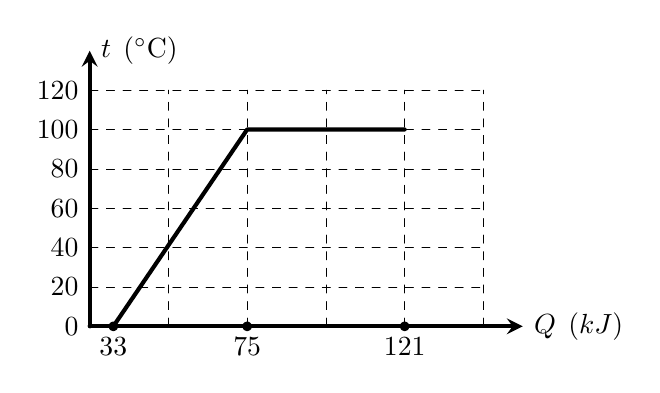
\begin{tikzpicture}[scale = 0.5, line join=round, line cap=round, >=stealth,line width=1.5]
			\draw[->, line width = 1.5] (0,0)--(0,7) node[right] {$t\;\left(^\circ \mathrm{C}\right)$};
			\draw[->, line width = 1.5] (0,0)--(11,0) node[right] {$Q\;\left(kJ\right)$};
			\draw[dashed,line width=0.2,xstep=2,ystep=1] (0,0) grid (10,6);
			\draw (0.6,0) -- (4,5) -- (8,5);
			\draw[fill=black] (0.6,0) circle (2pt) node [below] {$33$} (4,0) circle (2pt) node [below] {$75$} (8,0) circle (2pt) node [below] {$121$};
			\path (0,0) node [left] {$0$}
			(0,1) node [left] {$20$}
			(0,2) node [left] {$40$}
			(0,3) node [left] {$60$}
			(0,4) node [left] {$80$}
			(0,5) node [left] {$100$}
			(0,6) node [left] {$120$};
		\end{tikzpicture}
	}
	\choiceTF
	{Nhiệt lượng cung cấp cho quá trình hóa hơi của nước là $121\ \mathrm{kJ}$}
	{\True Từ khi nước đá nóng chảy hoàn toàn đến khi nước bắt đầu sôi, nước đã nhận nhiệt lượng $42\ \mathrm{kJ}$}
	{Khối lượng của nước đá ban đầu là $80\ \mathrm{g}$}
	{\True Đoạn BC cho biết lượng nước đã hóa hơi là $20\ \mathrm{g}$}
	\loigiai{
		\begin{itemchoice}
			\item Dựa vào đồ thị, quá trình hóa hơi xảy ra tại $100^\circ \mathrm{C}$ (đoạn nằm ngang cuối cùng). Nhiệt lượng cung cấp cho quá trình hóa hơi là $Q_{h} = 121 - 75 = 46\ \mathrm{kJ}$. Do đó phát biểu này sai.
			\item Nước đá nóng chảy hoàn toàn tại giá trị nhiệt lượng $Q_1 = 33\ \mathrm{kJ}$ và bắt đầu sôi tại giá trị nhiệt lượng $Q_2 = 75\ \mathrm{kJ}$. Từ đồ thị, nhiệt lượng nước đã nhận trong giai đoạn này là $\Delta Q = 75 - 33 = 42\ \mathrm{kJ}$. Do đó phát biểu này đúng.
			\item Áp dụng công thức tính nhiệt lượng nóng chảy: $Q = m \cdot \lambda$. Khối lượng của nước đá ban đầu là $m = \frac{Q}{\lambda} = \frac{33\,000}{3{,}3 \cdot 10^5} = 0{,}1\ \mathrm{kg} = 100\ \mathrm{g}$. Do đó phát biểu này sai.
			\item Áp dụng công thức tính nhiệt lượng hóa hơi: $Q_h = m' \cdot L$. Lượng nước đã hóa hơi (ứng với đoạn nằm ngang ở $100^\circ \mathrm{C}$) là $m' = \frac{Q_h}{L} = \frac{46\,000}{2{,}3 \cdot 10^6} = 0{,}02\ \mathrm{kg} = 20\ \mathrm{g}$. Do đó phát biểu này đúng.
		\end{itemchoice}
	}
\end{ex}

% ID: L12C1B1-TLN-10
% Mức: TH
% ID: L12C1B1-158-TLN
% ID: L12C1B1-158-TLN
% Mức: TH
% ID: L12C1B1-158-TLN
% Mức: TH
% ID: L12C1B1-158-TLN
% ID: L12C1B1-158-TLN
% Mức: TH
% ID: L12C1B1-158-TLN
% Mức: TH
% ID: L12C1B1-158-TLN
% ID: L12C1B1-158-TLN
% Mức: TH
% ID: L12C1B6-135-TLN
%=== Câu 71 ===%
\begin{bt}
% ID: L12C1B6-135-TLN
% Mức: TH
	{\color{red}\footnotesize\ttfamily [L12C1B1-TLN-10]}\par %HienID
	Một chất rắn kết tinh được đun nóng liên tục. Đồ thị nhiệt độ - thời gian cho thấy nhiệt độ tăng đều từ phút thứ $0$ đến phút thứ $5$ (từ $20^\circ\mathrm{C}$ đến $80^\circ\mathrm{C}$), sau đó giữ nguyên ở $80^\circ\mathrm{C}$ từ phút thứ $5$ đến phút thứ $12$ (đang nóng chảy), rồi tiếp tục tăng. Chất này nóng chảy ở nhiệt độ bao nhiêu độ $\mathrm{C}$?
	\shortans[oly]{$80$}
	\loigiai{
		Nhiệt độ nóng chảy của chất rắn kết tinh là giá trị nhiệt độ không đổi trong đoạn nằm ngang của đồ thị, ở đây là $80^\circ\mathrm{C}$.
	}
\end{bt}

% ID: L12C1B1-TLN-11
% Mức: TH
% ID: L12C1B1-159-TLN
% ID: L12C1B1-159-TLN
% Mức: TH
% ID: L12C1B1-159-TLN
% Mức: TH
% ID: L12C1B1-159-TLN
% ID: L12C1B1-159-TLN
% Mức: TH
% ID: L12C1B1-159-TLN
% Mức: TH
% ID: L12C1B1-159-TLN
% ID: L12C1B1-159-TLN
% Mức: TH
% ID: L12C1B6-136-TLN
%=== Câu 72 ===%
\begin{bt}
% ID: L12C1B6-136-TLN
% Mức: TH
	{\color{red}\footnotesize\ttfamily [L12C1B1-TLN-11]}\par %HienID
	Một khối nước đá đang tan hoàn toàn ở $0^\circ\mathrm{C}$ rồi được đun tiếp đến khi sôi ở $100^\circ\mathrm{C}$. Trên đồ thị nhiệt độ theo thời gian, đoạn ứng với quá trình nóng chảy là một đường nằm ngang tại giá trị nhiệt độ bao nhiêu độ $\mathrm{C}$?
	\shortans[oly]{$0$}
	\loigiai{
		Trong suốt quá trình nóng chảy, nhiệt độ của nước đá không đổi và bằng nhiệt độ nóng chảy của nước đá là $0^\circ\mathrm{C}$, nên đoạn đồ thị tương ứng là đường nằm ngang tại $0^\circ\mathrm{C}$.
	}
\end{bt}

% ===== Câu 108 =====
% ID: L12C1B1-27-TN
% Mức: NB

% ===== Câu 109 =====
% ID: L12C1B6-137-DS
% Mức: NB
\begin{ex}
% ID: L12C1B6-137-DS
% Mức: NB
Xét các phát biểu sau về dạng “Đọc và phân tích đồ thị quá trình chuyển thể” (bộ số 4).
\choiceTF
{\True Trong thời gian chất kết tinh tinh khiết nóng chảy ở áp suất không đổi, nhiệt độ không đổi.}
{Đoạn nằm ngang trên đường đun nóng luôn biểu diễn chất đang tăng nhiệt độ.}
{\True Khi giải dạng “Đọc và phân tích đồ thị quá trình chuyển thể”, cần xác định đúng trạng thái đầu, trạng thái cuối và quy ước dấu hoặc điều kiện áp dụng.}
{Có thể bỏ qua mọi dữ kiện về khối lượng, nhiệt độ và hiệu suất trong mọi bài toán thuộc dạng này.}
\loigiai{
\begin{itemchoice}
\item (Đúng) Trong thời gian chất kết tinh tinh khiết nóng chảy ở áp suất không đổi, nhiệt độ không đổi. (Vì): Trong thời gian chất kết tinh tinh khiết nóng chảy ở áp suất không đổi, nhiệt độ không đổi. b) S: Đoạn nằm ngang trên đường đun nóng luôn biểu diễn chất đang tăng nhiệt độ. c) Đ: Khi giải dạng “Đọc và phân tích đồ thị quá trình chuyển thể”, cần xác định đúng trạng thái đầu, trạng thái cuối và quy ước dấu hoặc điều kiện áp dụng. d) S: Có thể bỏ qua mọi dữ kiện về khối lượng, nhiệt độ và hiệu suất trong mọi bài toán thuộc dạng này. Kết luận dựa trên định nghĩa, điều kiện áp dụng và quy ước trong SGK KNTT
\item (Sai) Đoạn nằm ngang trên đường đun nóng luôn biểu diễn chất đang tăng nhiệt độ.
\item (Đúng) Khi giải dạng “Đọc và phân tích đồ thị quá trình chuyển thể”, cần xác định đúng trạng thái đầu, trạng thái cuối và quy ước dấu hoặc điều kiện áp dụng.
\item (Sai) Có thể bỏ qua mọi dữ kiện về khối lượng, nhiệt độ và hiệu suất trong mọi bài toán thuộc dạng này.
\end{itemchoice}
}
\end{ex}

% ===== Câu 113 =====
% ID: L12C1B6-138-DS
% Mức: TH
\begin{ex}
% ID: L12C1B6-138-DS
% Mức: TH
Xét các phát biểu sau về dạng “Đọc và phân tích đồ thị quá trình chuyển thể” (bộ số 1).
\choiceTF
{Đoạn nằm ngang trên đường đun nóng luôn biểu diễn chất đang tăng nhiệt độ.}
{\True Khi giải dạng “Đọc và phân tích đồ thị quá trình chuyển thể”, cần xác định đúng trạng thái đầu, trạng thái cuối và quy ước dấu hoặc điều kiện áp dụng.}
{Có thể bỏ qua mọi dữ kiện về khối lượng, nhiệt độ và hiệu suất trong mọi bài toán thuộc dạng này.}
{\True Trong thời gian chất kết tinh tinh khiết nóng chảy ở áp suất không đổi, nhiệt độ không đổi.}
\loigiai{
\begin{itemchoice}
\item (Sai) Đoạn nằm ngang trên đường đun nóng luôn biểu diễn chất đang tăng nhiệt độ. (Vì): Đoạn nằm ngang trên đường đun nóng luôn biểu diễn chất đang tăng nhiệt độ. b) Đ: Khi giải dạng “Đọc và phân tích đồ thị quá trình chuyển thể”, cần xác định đúng trạng thái đầu, trạng thái cuối và quy ước dấu hoặc điều kiện áp dụng. c) S: Có thể bỏ qua mọi dữ kiện về khối lượng, nhiệt độ và hiệu suất trong mọi bài toán thuộc dạng này. d) Đ: Trong thời gian chất kết tinh tinh khiết nóng chảy ở áp suất không đổi, nhiệt độ không đổi. Kết luận dựa trên định nghĩa, điều kiện áp dụng và quy ước trong SGK KNTT
\item (Đúng) Khi giải dạng “Đọc và phân tích đồ thị quá trình chuyển thể”, cần xác định đúng trạng thái đầu, trạng thái cuối và quy ước dấu hoặc điều kiện áp dụng.
\item (Sai) Có thể bỏ qua mọi dữ kiện về khối lượng, nhiệt độ và hiệu suất trong mọi bài toán thuộc dạng này.
\item (Đúng) Trong thời gian chất kết tinh tinh khiết nóng chảy ở áp suất không đổi, nhiệt độ không đổi.
\end{itemchoice}
}
\end{ex}

% ===== Câu 117 =====
% ID: L12C1B6-139-DS
% Mức: TH
\begin{ex}
% ID: L12C1B6-139-DS
% Mức: TH
Xét các phát biểu sau về dạng “Đọc và phân tích đồ thị quá trình chuyển thể” (bộ số 5).
\choiceTF
{Đoạn nằm ngang trên đường đun nóng luôn biểu diễn chất đang tăng nhiệt độ.}
{\True Khi giải dạng “Đọc và phân tích đồ thị quá trình chuyển thể”, cần xác định đúng trạng thái đầu, trạng thái cuối và quy ước dấu hoặc điều kiện áp dụng.}
{Có thể bỏ qua mọi dữ kiện về khối lượng, nhiệt độ và hiệu suất trong mọi bài toán thuộc dạng này.}
{\True Trong thời gian chất kết tinh tinh khiết nóng chảy ở áp suất không đổi, nhiệt độ không đổi.}
\loigiai{
\begin{itemchoice}
\item (Sai) Đoạn nằm ngang trên đường đun nóng luôn biểu diễn chất đang tăng nhiệt độ. (Vì): Đoạn nằm ngang trên đường đun nóng luôn biểu diễn chất đang tăng nhiệt độ. b) Đ: Khi giải dạng “Đọc và phân tích đồ thị quá trình chuyển thể”, cần xác định đúng trạng thái đầu, trạng thái cuối và quy ước dấu hoặc điều kiện áp dụng. c) S: Có thể bỏ qua mọi dữ kiện về khối lượng, nhiệt độ và hiệu suất trong mọi bài toán thuộc dạng này. d) Đ: Trong thời gian chất kết tinh tinh khiết nóng chảy ở áp suất không đổi, nhiệt độ không đổi. Kết luận dựa trên định nghĩa, điều kiện áp dụng và quy ước trong SGK KNTT
\item (Đúng) Khi giải dạng “Đọc và phân tích đồ thị quá trình chuyển thể”, cần xác định đúng trạng thái đầu, trạng thái cuối và quy ước dấu hoặc điều kiện áp dụng.
\item (Sai) Có thể bỏ qua mọi dữ kiện về khối lượng, nhiệt độ và hiệu suất trong mọi bài toán thuộc dạng này.
\item (Đúng) Trong thời gian chất kết tinh tinh khiết nóng chảy ở áp suất không đổi, nhiệt độ không đổi.
\end{itemchoice}
}
\end{ex}

% ===== Câu 121 =====
% ID: L12C1B6-140-DS
% Mức: VD
\begin{ex}
% ID: L12C1B6-140-DS
% Mức: VD
Xét các phát biểu sau về dạng “Đọc và phân tích đồ thị quá trình chuyển thể” (bộ số 2).
\choiceTF
{\True Khi giải dạng “Đọc và phân tích đồ thị quá trình chuyển thể”, cần xác định đúng trạng thái đầu, trạng thái cuối và quy ước dấu hoặc điều kiện áp dụng.}
{Có thể bỏ qua mọi dữ kiện về khối lượng, nhiệt độ và hiệu suất trong mọi bài toán thuộc dạng này.}
{\True Trong thời gian chất kết tinh tinh khiết nóng chảy ở áp suất không đổi, nhiệt độ không đổi.}
{Đoạn nằm ngang trên đường đun nóng luôn biểu diễn chất đang tăng nhiệt độ.}
\loigiai{
\begin{itemchoice}
\item (Đúng) Khi giải dạng “Đọc và phân tích đồ thị quá trình chuyển thể”, cần xác định đúng trạng thái đầu, trạng thái cuối và quy ước dấu hoặc điều kiện áp dụng. (Vì): Khi giải dạng “Đọc và phân tích đồ thị quá trình chuyển thể”, cần xác định đúng trạng thái đầu, trạng thái cuối và quy ước dấu hoặc điều kiện áp dụng. b) S: Có thể bỏ qua mọi dữ kiện về khối lượng, nhiệt độ và hiệu suất trong mọi bài toán thuộc dạng này. c) Đ: Trong thời gian chất kết tinh tinh khiết nóng chảy ở áp suất không đổi, nhiệt độ không đổi. d) S: Đoạn nằm ngang trên đường đun nóng luôn biểu diễn chất đang tăng nhiệt độ. Kết luận dựa trên định nghĩa, điều kiện áp dụng và quy ước trong SGK KNTT
\item (Sai) Có thể bỏ qua mọi dữ kiện về khối lượng, nhiệt độ và hiệu suất trong mọi bài toán thuộc dạng này.
\item (Đúng) Trong thời gian chất kết tinh tinh khiết nóng chảy ở áp suất không đổi, nhiệt độ không đổi.
\item (Sai) Đoạn nằm ngang trên đường đun nóng luôn biểu diễn chất đang tăng nhiệt độ.
\end{itemchoice}
}
\end{ex}

% ===== Câu 122 =====
% ID: L12C1B6-141-TL
% Mức: NB
\begin{bt}
% ID: L12C1B6-141-TL
% Mức: NB
Trình bày cách nhận biết và phương pháp giải dạng “Đọc và phân tích đồ thị quá trình chuyển thể”. Phân tích nhận định sau và sửa lại nếu sai: “Đoạn nằm ngang trên đường đun nóng luôn biểu diễn chất đang tăng nhiệt độ.”
\loigiai{
Trước hết xác định hiện tượng, trạng thái và các đại lượng đã cho. Nêu định nghĩa hoặc hệ thức phù hợp, đổi về đơn vị SI, áp dụng đúng điều kiện và kiểm tra ý nghĩa kết quả. Nhận định cần đối chiếu: Trong thời gian chất kết tinh tinh khiết nóng chảy ở áp suất không đổi, nhiệt độ không đổi. Vì vậy nhận định đã cho sai; phát biểu đúng là: Trong thời gian chất kết tinh tinh khiết nóng chảy ở áp suất không đổi, nhiệt độ không đổi.
}
\end{bt}

% ===== Câu 123 =====
% ID: L12C1B6-142-TLN
% Mức: NB
\begin{ex}
% ID: L12C1B6-142-TLN
% Mức: NB
Cho bốn nhận định: (1) Trong thời gian chất kết tinh tinh khiết nóng chảy ở áp suất không đổi, nhiệt độ không đổi. (2) Đoạn nằm ngang trên đường đun nóng luôn biểu diễn chất đang tăng nhiệt độ. (3) Cần kiểm tra đơn vị và điều kiện áp dụng khi xử lí dạng “Đọc và phân tích đồ thị quá trình chuyển thể”. (4) Có thể thay tùy ý nhiệt độ Celsius cho nhiệt độ tuyệt đối trong mọi công thức. Có bao nhiêu nhận định đúng? Trả lời bằng một số nguyên.
\shortans{2}
\loigiai{
Nhận định (1) và (3) đúng; (2) và (4) sai. Vậy có 2 nhận định đúng.
}
\end{ex}

% ===== Câu 125 =====
% ID: L12C1B6-143-DS
% Mức: VDC
\begin{ex}
% ID: L12C1B6-143-DS
% Mức: VDC
Xét các phát biểu sau về dạng “Đọc và phân tích đồ thị quá trình chuyển thể” (bộ số 3).
\choiceTF
{Có thể bỏ qua mọi dữ kiện về khối lượng, nhiệt độ và hiệu suất trong mọi bài toán thuộc dạng này.}
{\True Trong thời gian chất kết tinh tinh khiết nóng chảy ở áp suất không đổi, nhiệt độ không đổi.}
{Đoạn nằm ngang trên đường đun nóng luôn biểu diễn chất đang tăng nhiệt độ.}
{\True Khi giải dạng “Đọc và phân tích đồ thị quá trình chuyển thể”, cần xác định đúng trạng thái đầu, trạng thái cuối và quy ước dấu hoặc điều kiện áp dụng.}
\loigiai{
\begin{itemchoice}
\item (Sai) Có thể bỏ qua mọi dữ kiện về khối lượng, nhiệt độ và hiệu suất trong mọi bài toán thuộc dạng này. (Vì): Có thể bỏ qua mọi dữ kiện về khối lượng, nhiệt độ và hiệu suất trong mọi bài toán thuộc dạng này. b) Đ: Trong thời gian chất kết tinh tinh khiết nóng chảy ở áp suất không đổi, nhiệt độ không đổi. c) S: Đoạn nằm ngang trên đường đun nóng luôn biểu diễn chất đang tăng nhiệt độ. d) Đ: Khi giải dạng “Đọc và phân tích đồ thị quá trình chuyển thể”, cần xác định đúng trạng thái đầu, trạng thái cuối và quy ước dấu hoặc điều kiện áp dụng. Kết luận dựa trên định nghĩa, điều kiện áp dụng và quy ước trong SGK KNTT
\item (Đúng) Trong thời gian chất kết tinh tinh khiết nóng chảy ở áp suất không đổi, nhiệt độ không đổi.
\item (Sai) Đoạn nằm ngang trên đường đun nóng luôn biểu diễn chất đang tăng nhiệt độ.
\item (Đúng) Khi giải dạng “Đọc và phân tích đồ thị quá trình chuyển thể”, cần xác định đúng trạng thái đầu, trạng thái cuối và quy ước dấu hoặc điều kiện áp dụng.
\end{itemchoice}
}
\end{ex}

% ===== Câu 129 =====
% ID: L12C1B6-144-TL
% Mức: TH
\begin{bt}
% ID: L12C1B6-144-TL
% Mức: TH
Trình bày cách nhận biết và phương pháp giải dạng “Đọc và phân tích đồ thị quá trình chuyển thể”. Phân tích nhận định sau và sửa lại nếu sai: “Trong thời gian chất kết tinh tinh khiết nóng chảy ở áp suất không đổi, nhiệt độ không đổi.”
\loigiai{
Trước hết xác định hiện tượng, trạng thái và các đại lượng đã cho. Nêu định nghĩa hoặc hệ thức phù hợp, đổi về đơn vị SI, áp dụng đúng điều kiện và kiểm tra ý nghĩa kết quả. Nhận định cần đối chiếu: Trong thời gian chất kết tinh tinh khiết nóng chảy ở áp suất không đổi, nhiệt độ không đổi. Vì vậy nhận định đã cho đúng.
}
\end{bt}

% ===== Câu 185 =====
% ID: L12C1B6-145-TN
% Mức: NB
\begin{ex}
% ID: L12C1B6-145-TN
% Mức: NB
Câu 1 thuộc dạng “Đọc và phân tích đồ thị quá trình chuyển thể”. Phát biểu nào sau đây đúng?
\choice
{Đoạn nằm ngang trên đường đun nóng luôn biểu diễn chất đang tăng nhiệt độ.}
{Nhiệt lượng và nhiệt độ là hai đại lượng hoàn toàn giống nhau.}
{Mọi quá trình nhiệt học đều không phụ thuộc điều kiện thực hiện.}
{\True Trong thời gian chất kết tinh tinh khiết nóng chảy ở áp suất không đổi, nhiệt độ không đổi.}
\loigiai{
Phát biểu đúng là: Trong thời gian chất kết tinh tinh khiết nóng chảy ở áp suất không đổi, nhiệt độ không đổi. Các phương án còn lại trái với mô hình, định nghĩa hoặc hệ thức nhiệt học tương ứng.
}
\end{ex}

% ===== Câu 186 =====
% ID: L12C1B6-146-TN
% Mức: NB
\begin{ex}
% ID: L12C1B6-146-TN
% Mức: NB
Câu 5 thuộc dạng “Đọc và phân tích đồ thị quá trình chuyển thể”. Phát biểu nào sau đây đúng?
\choice
{Đoạn nằm ngang trên đường đun nóng luôn biểu diễn chất đang tăng nhiệt độ.}
{Nhiệt lượng và nhiệt độ là hai đại lượng hoàn toàn giống nhau.}
{Mọi quá trình nhiệt học đều không phụ thuộc điều kiện thực hiện.}
{\True Trong thời gian chất kết tinh tinh khiết nóng chảy ở áp suất không đổi, nhiệt độ không đổi.}
\loigiai{
Phát biểu đúng là: Trong thời gian chất kết tinh tinh khiết nóng chảy ở áp suất không đổi, nhiệt độ không đổi. Các phương án còn lại trái với mô hình, định nghĩa hoặc hệ thức nhiệt học tương ứng.
}
\end{ex}

% ===== Câu 187 =====
% ID: L12C1B6-147-TN
% Mức: NB
\begin{ex}
% ID: L12C1B6-147-TN
% Mức: NB
Câu 9 thuộc dạng “Đọc và phân tích đồ thị quá trình chuyển thể”. Phát biểu nào sau đây đúng?
\choice
{Đoạn nằm ngang trên đường đun nóng luôn biểu diễn chất đang tăng nhiệt độ.}
{Nhiệt lượng và nhiệt độ là hai đại lượng hoàn toàn giống nhau.}
{Mọi quá trình nhiệt học đều không phụ thuộc điều kiện thực hiện.}
{\True Trong thời gian chất kết tinh tinh khiết nóng chảy ở áp suất không đổi, nhiệt độ không đổi.}
\loigiai{
Phát biểu đúng là: Trong thời gian chất kết tinh tinh khiết nóng chảy ở áp suất không đổi, nhiệt độ không đổi. Các phương án còn lại trái với mô hình, định nghĩa hoặc hệ thức nhiệt học tương ứng.
}
\end{ex}

% ===== Câu 188 =====
% ID: L12C1B6-148-TN
% Mức: TH
\begin{ex}
% ID: L12C1B6-148-TN
% Mức: TH
Câu 2 thuộc dạng “Đọc và phân tích đồ thị quá trình chuyển thể”. Phát biểu nào sau đây đúng?
\choice
{Nhiệt lượng và nhiệt độ là hai đại lượng hoàn toàn giống nhau.}
{Mọi quá trình nhiệt học đều không phụ thuộc điều kiện thực hiện.}
{\True Trong thời gian chất kết tinh tinh khiết nóng chảy ở áp suất không đổi, nhiệt độ không đổi.}
{Đoạn nằm ngang trên đường đun nóng luôn biểu diễn chất đang tăng nhiệt độ.}
\loigiai{
Phát biểu đúng là: Trong thời gian chất kết tinh tinh khiết nóng chảy ở áp suất không đổi, nhiệt độ không đổi. Các phương án còn lại trái với mô hình, định nghĩa hoặc hệ thức nhiệt học tương ứng.
}
\end{ex}

% ===== Câu 189 =====
% ID: L12C1B6-149-TN
% Mức: TH
\begin{ex}
% ID: L12C1B6-149-TN
% Mức: TH
Câu 6 thuộc dạng “Đọc và phân tích đồ thị quá trình chuyển thể”. Phát biểu nào sau đây đúng?
\choice
{Nhiệt lượng và nhiệt độ là hai đại lượng hoàn toàn giống nhau.}
{Mọi quá trình nhiệt học đều không phụ thuộc điều kiện thực hiện.}
{\True Trong thời gian chất kết tinh tinh khiết nóng chảy ở áp suất không đổi, nhiệt độ không đổi.}
{Đoạn nằm ngang trên đường đun nóng luôn biểu diễn chất đang tăng nhiệt độ.}
\loigiai{
Phát biểu đúng là: Trong thời gian chất kết tinh tinh khiết nóng chảy ở áp suất không đổi, nhiệt độ không đổi. Các phương án còn lại trái với mô hình, định nghĩa hoặc hệ thức nhiệt học tương ứng.
}
\end{ex}

% ===== Câu 190 =====
% ID: L12C1B6-150-TN
% Mức: TH
\begin{ex}
% ID: L12C1B6-150-TN
% Mức: TH
Câu 10 thuộc dạng “Đọc và phân tích đồ thị quá trình chuyển thể”. Phát biểu nào sau đây đúng?
\choice
{Nhiệt lượng và nhiệt độ là hai đại lượng hoàn toàn giống nhau.}
{Mọi quá trình nhiệt học đều không phụ thuộc điều kiện thực hiện.}
{\True Trong thời gian chất kết tinh tinh khiết nóng chảy ở áp suất không đổi, nhiệt độ không đổi.}
{Đoạn nằm ngang trên đường đun nóng luôn biểu diễn chất đang tăng nhiệt độ.}
\loigiai{
Phát biểu đúng là: Trong thời gian chất kết tinh tinh khiết nóng chảy ở áp suất không đổi, nhiệt độ không đổi. Các phương án còn lại trái với mô hình, định nghĩa hoặc hệ thức nhiệt học tương ứng.
}
\end{ex}

% ===== Câu 191 =====
% ID: L12C1B6-151-TN
% Mức: VD
\begin{ex}
% ID: L12C1B6-151-TN
% Mức: VD
Câu 3 thuộc dạng “Đọc và phân tích đồ thị quá trình chuyển thể”. Phát biểu nào sau đây đúng?
\choice
{Mọi quá trình nhiệt học đều không phụ thuộc điều kiện thực hiện.}
{\True Trong thời gian chất kết tinh tinh khiết nóng chảy ở áp suất không đổi, nhiệt độ không đổi.}
{Đoạn nằm ngang trên đường đun nóng luôn biểu diễn chất đang tăng nhiệt độ.}
{Nhiệt lượng và nhiệt độ là hai đại lượng hoàn toàn giống nhau.}
\loigiai{
Phát biểu đúng là: Trong thời gian chất kết tinh tinh khiết nóng chảy ở áp suất không đổi, nhiệt độ không đổi. Các phương án còn lại trái với mô hình, định nghĩa hoặc hệ thức nhiệt học tương ứng.
}
\end{ex}

% ===== Câu 192 =====
% ID: L12C1B6-152-TN
% Mức: VD
\begin{ex}
% ID: L12C1B6-152-TN
% Mức: VD
Câu 7 thuộc dạng “Đọc và phân tích đồ thị quá trình chuyển thể”. Phát biểu nào sau đây đúng?
\choice
{Mọi quá trình nhiệt học đều không phụ thuộc điều kiện thực hiện.}
{\True Trong thời gian chất kết tinh tinh khiết nóng chảy ở áp suất không đổi, nhiệt độ không đổi.}
{Đoạn nằm ngang trên đường đun nóng luôn biểu diễn chất đang tăng nhiệt độ.}
{Nhiệt lượng và nhiệt độ là hai đại lượng hoàn toàn giống nhau.}
\loigiai{
Phát biểu đúng là: Trong thời gian chất kết tinh tinh khiết nóng chảy ở áp suất không đổi, nhiệt độ không đổi. Các phương án còn lại trái với mô hình, định nghĩa hoặc hệ thức nhiệt học tương ứng.
}
\end{ex}

% ===== Câu 193 =====
% ID: L12C1B6-153-TN
% Mức: VDC
\begin{ex}
% ID: L12C1B6-153-TN
% Mức: VDC
Câu 4 thuộc dạng “Đọc và phân tích đồ thị quá trình chuyển thể”. Phát biểu nào sau đây đúng?
\choice
{\True Trong thời gian chất kết tinh tinh khiết nóng chảy ở áp suất không đổi, nhiệt độ không đổi.}
{Đoạn nằm ngang trên đường đun nóng luôn biểu diễn chất đang tăng nhiệt độ.}
{Nhiệt lượng và nhiệt độ là hai đại lượng hoàn toàn giống nhau.}
{Mọi quá trình nhiệt học đều không phụ thuộc điều kiện thực hiện.}
\loigiai{
Phát biểu đúng là: Trong thời gian chất kết tinh tinh khiết nóng chảy ở áp suất không đổi, nhiệt độ không đổi. Các phương án còn lại trái với mô hình, định nghĩa hoặc hệ thức nhiệt học tương ứng.
}
\end{ex}

% ===== Câu 194 =====
% ID: L12C1B6-154-TN
% Mức: VDC
\begin{ex}
% ID: L12C1B6-154-TN
% Mức: VDC
Câu 8 thuộc dạng “Đọc và phân tích đồ thị quá trình chuyển thể”. Phát biểu nào sau đây đúng?
\choice
{\True Trong thời gian chất kết tinh tinh khiết nóng chảy ở áp suất không đổi, nhiệt độ không đổi.}
{Đoạn nằm ngang trên đường đun nóng luôn biểu diễn chất đang tăng nhiệt độ.}
{Nhiệt lượng và nhiệt độ là hai đại lượng hoàn toàn giống nhau.}
{Mọi quá trình nhiệt học đều không phụ thuộc điều kiện thực hiện.}
\loigiai{
Phát biểu đúng là: Trong thời gian chất kết tinh tinh khiết nóng chảy ở áp suất không đổi, nhiệt độ không đổi. Các phương án còn lại trái với mô hình, định nghĩa hoặc hệ thức nhiệt học tương ứng.
}
\end{ex}
